\chapter{Escenario del Problema}
\begin{figure}[H]
\centering
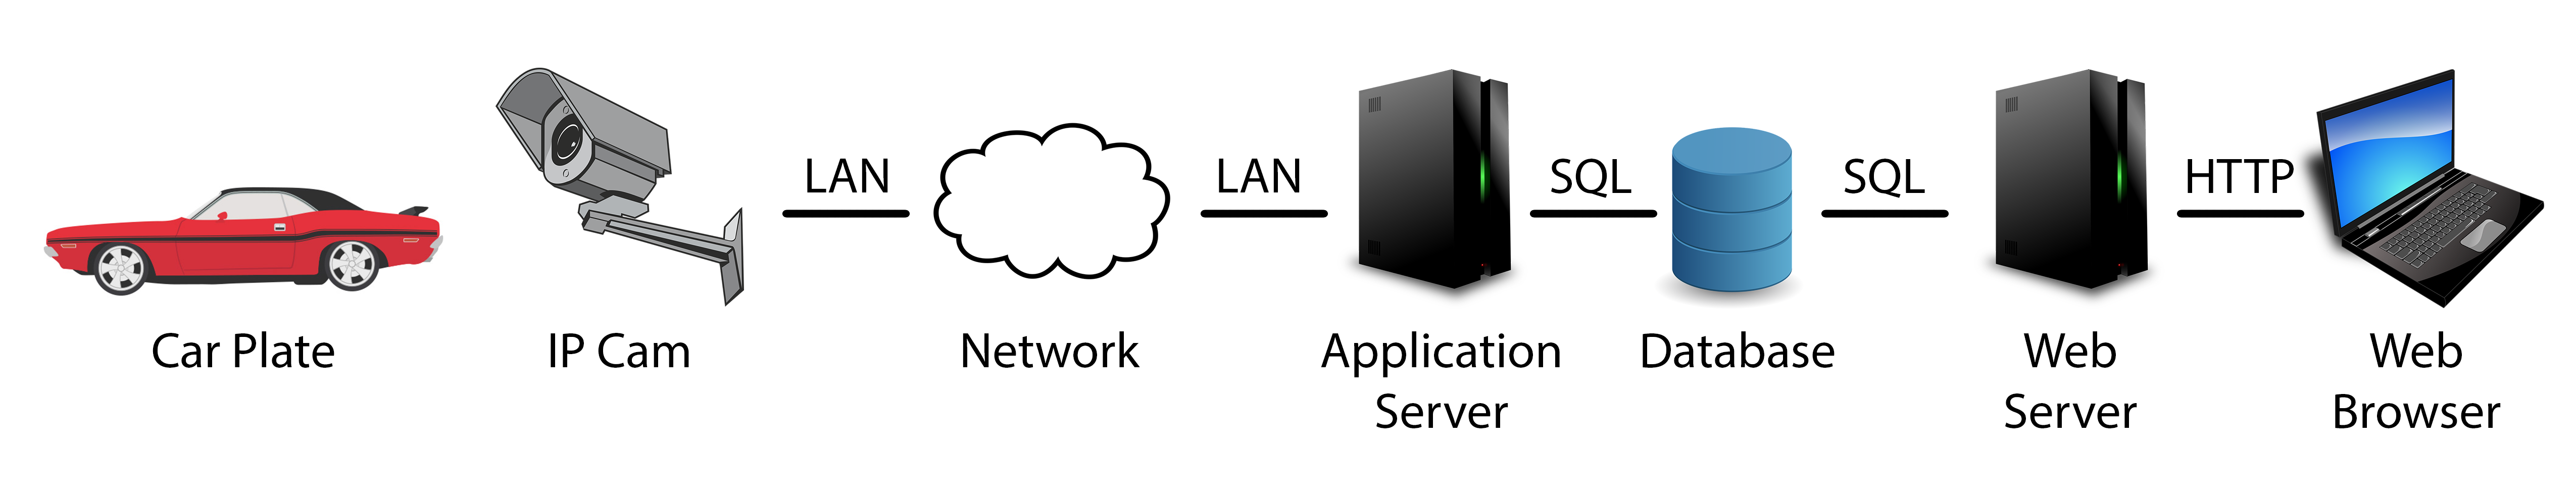
\includegraphics[width=0.90\textwidth]{nodos-overview}
\caption{Panorama de los Nodos de la Aplicación}
\label{fig:nodos-overview}
\end{figure}
    
    Como se observa en la Figura \ref{fig:nodos-overview}, la aplicación distribuirá el nodo de aplicación, donde se ejecutaran los servicios; el servidor de la base de datos; y, el servidor web, a través del cual el usuario accede a la información relacionada a los registros y al sistema.
        
    El proceso de reconocimiento de una matrícula sigue la siguiente cadena de procesos:

        \begin{enumerate}
            \item Existe una cámara instalada y la información de la misma se encuentra almacenada en la base de datos.
            \item El Servicio de Recolección de vídeo, una vez iniciado, reenvía el flujo de vídeo (cuadros) a un LB.
            \item El LB distribuye los cuadros de vídeo recibidos entre los servicios de Reconocimiento disponibles.
            \item El Servicio de Reconocimiento, por cada cuadro, ejecuta el algoritmo de reconocimiento y reenvía las coincidencias o matriculas reconocidas a el Servicio de Coincidencias.
            \item el servicio de coincidencias guarda en la BD las  o matriculas reconocidas, independiente de si se encuentra un propietario asociado o no.
        \end{enumerate}    
        
Toda la información de las matriculas reconocidas puede verse desde el cliente web.

Bajo esquema de la Figura \ref{fig:nodos-arch}, los servicios que componen a la aplicación pueden ser categorizados en

    \begin{itemize}
        \item Servicios Atómicos: IaaS, Cámara, Matricula, Lugar, Propietario, Coincidencias, Base de Datos, LB
        \item Servicios Compuestos: Servicio Recolector, Servicio de Reconocimiento, Servicio Web
    \end{itemize}
    De igual manera, pueden ser categorizados según su rol en la aplicación:
    \begin{itemize}
        \item Servicios Clave: Servicio Recolector, Servicio de Reconocimiento, Cámara, Matricula, Lugar, Propietario, Coincidencia
        \item Servicios de Soporte: Servicio Web, LB, IaaS, Servicio Web
    \end{itemize}

\begin{figure}[ht]
\centering
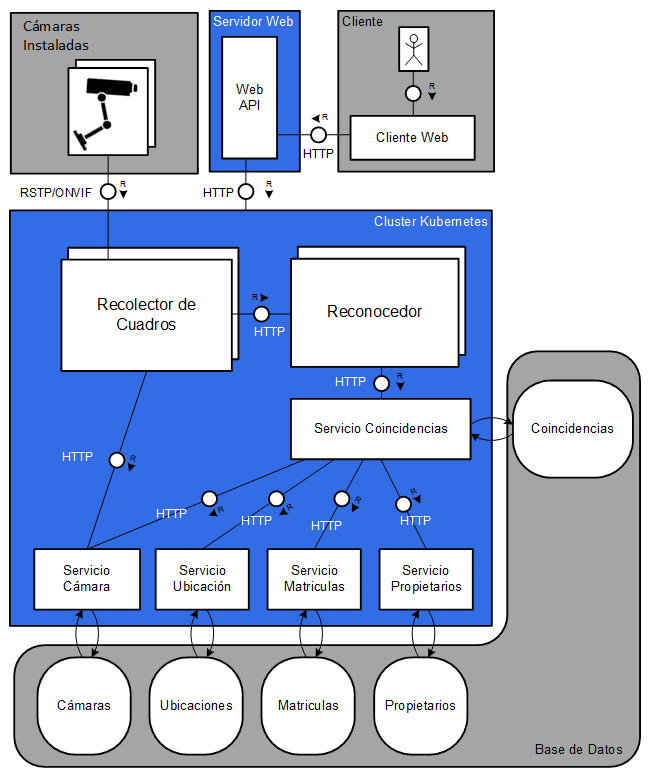
\includegraphics[width=.75\textwidth]{nodos-arch2}
\caption{Arquitectura de la Aplicación}
\label{fig:nodos-arch}
\end{figure} 